\section{Robustness Test}
\label{sec:robustness}
Three alternative settings are used to test the baseline result regarding the investment demand shock---the first one uses the standard \cite{smetsShocksFrictionsUS2007} model; the second discusses the case where the investment demand shock is i.i.d.; the last one further differentiates the IST shock and the marginal efficiency of investment (MEI) shock, following \cite{justinianoInvestmentShocksRelative2011}.

\subsection{Smets--Wouters-style Model}
\label{sec:robustness:sw}
In this section, the baseline model is expanded following \cite{smetsShocksFrictionsUS2007} to address the underlying concerns of oversimplification. Specifically, I add a habit formation term in the utility function and a monopolistic competition structure in the labor market. In addition, a preference shock, a price markup shock and a wage markup shock are added as well. In terms of data, the consumption and wage growth rates are added.

The utility function of households becomes
\begin{equation}
    \mathbb{E}_t \left[ \sum_{s=0}^{\infty} \beta^s \mu_{b, t+s} \left( \ln(C_{t+s} - h C_{t+s-1}) - \chi \frac{L_{t+s}(j)^{1+\psi}}{1+\psi} \right) \right],
\end{equation}
where $\mu_{b, t}$ is the intertemporal preference shock, following
\begin{equation}
    \ln \mu_{b, t} = (1 - \rho_b) \mu_b + \rho_b \ln \mu_{b, t-1} + \varepsilon_{b, t}, \,\, \varepsilon_{b, t}\sim \text{i.i.d. } N (0, \sigma_b^2).
\end{equation}

It is worth to mention that the consumption part in the utility function becomes logarithmic instead of the more general CRRA form. This is because with habit formation and separable utility function between $C_t$ and $L_t$, general CRRA utility function doesn't have a balanced growth path unless it reduces to a logarithmic form.

The stochastic discount factor becomes
\begin{equation}
    SDF_t = \beta \left(\frac{c_{t+1} - hc_t}{c_t - hc_{t-1}}\right)^{-1} = \beta \left(\frac{\gamma \tilde{c}_{t+1} - h\tilde{c}_t}{\tilde{c}_t - \frac{h}{\gamma}\tilde{c}_{t-1}}\right)^{-1},
\end{equation}
where $\tilde{c}_t = c_t / \gamma^t$ is the detrended variable.

The labor market and wage Calvo pricing problem follow \cite{erceg2000optimal}, which gives us the wage Phillips curve
\begin{equation}
    \hat{\pi}_t^w = \beta \mathbb{E}_t \hat{\pi}_{t+1}^w - \kappa_w \left(\hat{w}_t - \hat{MRS}_t\right) + \mu_{w, t},
\end{equation}
where $\kappa_w = \frac{(1 - \theta_w)(1 - \beta\theta_w)}{\theta_w(1+\nu_{w} \psi)}$. Because of the weak identification problem \footnote{$\nu_w$, $\theta_w$ only play a role in $\kappa_w$, but $\kappa_w$ can be the same under different value combinations of $\nu_w$ and $\theta_w$. Thus the model will be unable to identify $\nu_w$ and $\theta_w$ parameters separately.}, $\nu_w$ is set as $3$ following \cite{smetsShocksFrictionsUS2007}.

$\mu_{w, t}$ is the wage markup shock following
\begin{equation}
    \ln \mu_{w, t} = (1 - \rho_w) \mu_w + \rho_w \ln \mu_{w, t-1} + \varepsilon_{w, t}, \,\, \varepsilon_{w, t}\sim \text{i.i.d. } N (0, \sigma_w^2).
\end{equation}

The price markup shock $\mu_{p, t}$ is added in the same way---right after the Phillips curve. I assume the markup shocks follow AR(1) processes for simplicity, while \cite{smetsShocksFrictionsUS2007} uses ARMA(1, 1) processes for these two shocks.

Two added observation equations are
\begin{equation}
    \begin{bmatrix}
        \Delta \ln CONS_t\\
        \Delta \ln WAGE_t
    \end{bmatrix}
    = 
    \begin{bmatrix}
        \bar{\gamma}\\
        \bar{\gamma}
    \end{bmatrix}
    +
    \begin{bmatrix}
        \hat{c}_t - \hat{c}_{t-1} \\
        \hat{w}_t - \hat{w}_{t-1}
    \end{bmatrix}
    +
    \Sigma_t^{meas}.
\end{equation}

Posteriors can be found in Table~\ref{tab:posterior-params:sw-type-no-rel} in Appendix \ref{app:result:sw}. Especially, both the Phillips curve and the wage Phillips curve become very flat, with $\kappa_p$ estimated as $0.03$ and $\kappa_w$ roughly $0.02$, which are much stickier than in the baseline result. A simple test that mutes the price and wage markup shocks shows that the low $\kappa_p$ and $\kappa_w$ partially benefit from these shocks, as they can alter price and wage exogenously, even though the endogenous part is rather sticky. The moments comparison is shown in Table~\ref{tab:varcmp:sw-type-no-rel}. As explained in Section~\ref{sec:results:moments}, the variance of hours worked is fitted much better.

It is clear that the investment demand shock has only a marginal effect on various macroeconomic variables, as shown in Table~\ref{tab:vd:sw-type-no-rel}. The investment demand shock can only contribute $4.37\%$ of the output forecast variance and $13.62\%$ of investment, and can hardly explain other variables such as inflation. Thus I flag the fragility of the baseline result in Table~\ref{tab:fevd-frequency:gov-data}.

% Auto-generated by test_variance_decomp_nocap.m
% file_name: sw_type_no_rel

\begin{table}[!htbp]
\centering
\caption{Unconditional FEVD (\%): Smets--Wouters-style model.}
\label{tab:vd:sw-type-no-rel}
\begin{tabular}{l r r r r r r r r}
\hline
Observable & $\varepsilon_g$ & $\varepsilon_{s}$ & $\varepsilon_R$ & $\varepsilon_a$ & $\varepsilon_b$ & $\varepsilon_p$ & $\varepsilon_w$ & $\varepsilon_{d}$ \\ 
\hline
Output & 6.15 & 10.31 & 7.86 & 43.58 & 17.21 & 5.00 & 5.52 & 4.37 \\ 
Inflation & 0.05 & 1.78 & 0.82 & 18.85 & 0.40 & 53.05 & 25.04 & 0.00 \\ 
Interest rate & 0.19 & 7.16 & 30.37 & 26.67 & 4.51 & 10.39 & 20.72 & 0.00 \\ 
Hours & 2.00 & 20.43 & 7.10 & 34.85 & 7.86 & 1.10 & 26.35 & 0.30 \\ 
Investment & 0.25 & 54.98 & 2.43 & 18.59 & 3.19 & 0.62 & 6.33 & 13.62 \\ 
Wage & 0.00 & 0.12 & 0.14 & 18.25 & 0.30 & 16.96 & 64.23 & 0.00 \\ 
Consumption & 0.25 & 2.36 & 6.48 & 43.49 & 42.01 & 1.92 & 3.49 & 0.00 \\ 
Gov. spending & 99.90 & 0.01 & 0.01 & 0.05 & 0.02 & 0.01 & 0.01 & 0.00 \\ 
\hline
\end{tabular}
\end{table}


Figure~\ref{fig:irf:sw} plots the IRF of the same state variables with the IRF of baseline result. There are three points that are different from the baseline result in Figure~\ref{fig:compare_irf}. First, investment demand shock generates much less fluctuation than IST shock due to the smaller standard deviation; second, IST shock now generates inflationary result, and the positive wage impact as well; third, consumption impact under investment demand shock becomes smoother---consumption impact is only $0.2\%$ of investment impact, whereas it is $12\%$ in the baseline result.

\begin{figure}
    \centering
    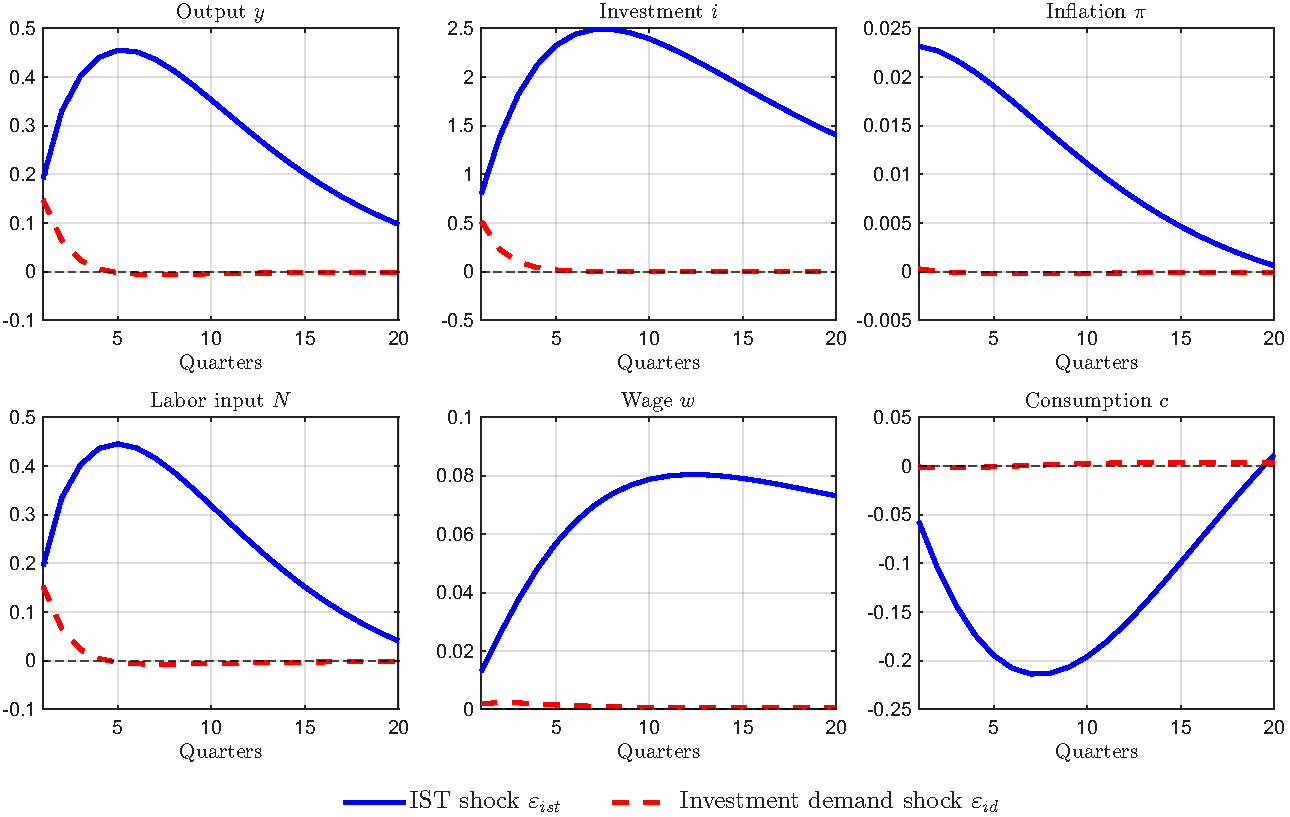
\includegraphics[width=0.9\textwidth]{figures/compare_irf_sw_type_no_rel.pdf}
    \caption{Impulse responses of output, investment, inflation, labor input, wage, and consumption to one-standard-deviation IST and investment demand shocks (Smets--Wouters-style model; horizon: 20 quarters).}
    \label{fig:irf:sw}
\end{figure}

I revisit the consumption impact in Figure~\ref{fig:sw:con}. Compared with the similar exercise in baseline result (Figure~\ref{fig:inv_demand_c1_kappa_psipi_heatmap}), I choose the parameters, the inverse Frisch elasticity $\psi$ and Taylor-rule output-gap coefficient $\psi_y$, to be varied. This is because the Phillips curve, as well as the wage Phillips curve, becomes quite flat. Thus, the slopes themselves have already approached to the \cite{nireiOriginsPropagationAnimal} calibration, and further, the inflation feedback in the Taylor's rule becomes less important because inflation hardly moves. However, the logic keeps the same---consumption impact is decided by the path of real interest rate, so nominal interest rate helps. If nominal interest rate is low enough, real interest can also be very low, and thus intertemporal substitution effect will be tempered. Smaller $\psi_y$ explicitly does this job by lowering output gap feedback in Taylor's rule. Smaller $\psi$ works through the output gap by suppressing the real wage---because nominal wage is very stikcy, the wage gap is smaller if real wage barely moves, and thus the output gap becomes smaller.
\begin{figure}
    \centering
    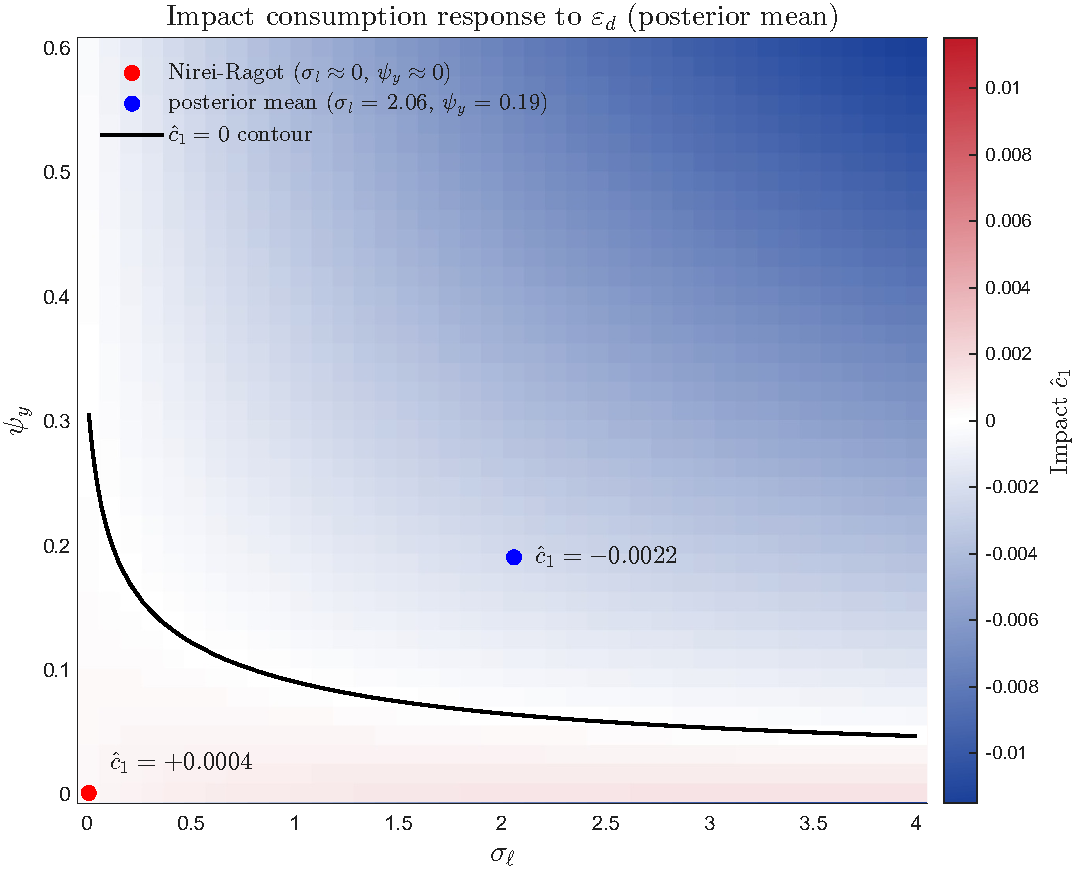
\includegraphics[width=0.7\textwidth]{figures/inv_demand_c1_psiy_sigmal_heatmap.pdf}
    \caption{Impact consumption response \(\hat c_1\) to a unit investment-demand shock as a function of the inverse Frisch elasticity \(\psi\) and the Taylor-rule output-gap coefficient \(\psi_y\). All other parameters are held at the posterior mean. }
    \label{fig:sw:con}
\end{figure}

Altogether, this section shows the sensitivity of the baseline result under an alternative model setting. However, its result can still be understood from the mechanisms analyzed in Section~\ref{sec:results}.

\subsection{Independent Investment Demand Shock}
\label{sec:robustness:iid}
Although using an AR(1) process to specify shocks is standard, it is natural to think that households will realize the exogenous investment demand in the $t+1$ period, and thus adjust their investment decision in $t+1$ to dampen the effect of the investment demand shock. Equivalently, this is to say that the investment demand shock only has a transitory effect in period $t$, which motivates the exercise in this section.

All other settings are unchanged compared with the baseline, except that $\rho_d$ is manually set as $0$. To be concise, I only present the FEVD result here in Table~\ref{tab:varcmp:per-add-mei}, and others can be found in Table~\ref{tab:posterior-params:per-add-mei} and Table~\ref{tab:varcmp:per-add-mei} in Appendix~\ref{app:result:iid}.

% Auto-generated by test_variance_decomp_nocap.m
% file_name: per_add_mei

\begin{table}[!htbp]
\centering
\caption{Variance decomposition (\%).}
\label{tab:vd:per-add-mei}
\begin{tabular}{l r r r r r}
\hline
Observable & $\varepsilon_g$ & $\varepsilon_{s}$ & $\varepsilon_R$ & $\varepsilon_a$ & $\varepsilon_{d}$ \\ 
\hline
Output & 6.67 & 38.60 & 9.35 & 22.42  & 22.95 \\ 
Inflation & 0.40 & 52.00 & 12.87 & 34.37 & 0.37 \\ 
Interest rate & 0.37 & 74.14 & 3.74 & 21.66 & 0.09 \\ 
Hours & 2.84 & 92.22 & 0.12 & 4.53 & 0.29 \\ 
Investment & 0.25 & 73.06 & 0.20 & 11.31 & 15.18 \\ 
Gov. spending & 99.59 & 0.17 & 0.04 & 0.10 & 0.10 \\ 
\hline
\end{tabular}
\end{table}


The investment demand shock contributes $22.95\%$ of output and $15.18\%$ of investment forecast error variance. Compared with the baseline result in Table~\ref{tab:fevd-frequency:gov-data}, the influence of the investment demand shock also decreases as expected, since the zero persistence cuts off the future influence.

\subsection{Marginal Efficiency of Investment Shock}
\label{sec:robustness:mei}
The topic in this section is subtle---it further distinguishes the IST shock from the marginal efficiency of investment (MEI) shock. Specifically, the IST shock means the efficiency from consumption goods to investment goods, and the MEI shock means the efficiency from investment goods to capital. However, without modelling the detailed investment goods producers and capital producers, both shocks stay in the capital law of motion in their reduced form,
\begin{equation}\label{eq:mei}
    k_{t+1} = (1 - \delta) k_t + \mu_{s, t}\mu_{m, t}\left[1 - S\left(\frac{i_t}{i_{t-1}}\right)\right] i_t,
\end{equation}
and thus there will be weak identification problem within the previous data set.

This test is motivated by \cite{justinianoInvestmentShocksRelative2011}, who claim that the IST shock will become less important if it is identified by data, and that the MEI shock becomes the one that matters. However, this raises a doubt about the estimation result---is the important thing just the residual in the capital law of motion? Although we can write multiple shocks in the capital law of motion, the equation suffers from a misspecification problem, in that we cannot be sure what the real shocks are. We can claim an IST shock, an investment demand shock, or an MEI shock in the capital law of motion, but which shocks to add depends on our assumptions. If the data-identified shock is less important, then the other part may be just the residual in the equation, and it is significant no matter what shock is named.

To alleviate the concern, the best thing to do is to identify the investment shock directly by some data. However, as this shock originates from idiosyncratic productivity shocks, the micro data that we need can hardly be incorporated into the current framework, where we only consider aggregate variables. Therefore, I can only conduct a horse-race test in this section by adding the MEI shock into the model. The result cannot conclusively establish the importance of the investment demand shock, but only offer some suggestions.

I use the relative price data to solve the weak identification problem mentioned in equation \eqref{eq:mei}. As pointed out by \cite{greenwoodLongRunImplicationsInvestmentSpecific1997a} and \cite{fisherDynamicEffectsNeutral2006}, the relative price of investment reflects the investment specific technology level in a one-sector model \footnote{If we model the production of consumption goods and investment goods as two sectors, such as in \cite{mouraInvestmentShocksSticky2018}, the relative price of investment goods is represented as the relative productivity, markup and marginal cost between these two sectors. Therefore, the relative price should have more complex dynamics in a more realistic model, rather than being only an exogenous stochastic process.}. Therefore, using the detrended relative price data, I assume that the detrended relative price represents the inverse of the IST level state variable. The data, the relative price of investment goods (PIRIC), is collected from FRED, and then I take $100\ln PIRIC_t$. As the data has an obvious trend, it should be detrended to match the model assumption that the logarithm of the IST level is a stationary process. Although it is more realistic to model the logarithm of IST level as a random walk process given the data, such modeling requires recalculating the balanced growth path, steady state and log-linearized model, as another growth term is added into the model. Thus, using the detrended data is a more straightforward approach.

% Auto-generated by test_variance_decomp_nocap.m
% file_name: para_add_mei

\begin{table}[!htbp]
\centering
\caption{Variance decomposition (\%).}
\label{tab:vd:para-add-mei}
\begin{tabular}{l r r r r r r}
\hline
Observable & $\varepsilon_g$ & $\varepsilon_{s}$ & $\varepsilon_R$ & $\varepsilon_a$ & $\varepsilon_{m}$ & $\varepsilon_{d}$ \\ 
\hline
Output & 4.58 & 0.44 & 10.81 & 23.79 & 17.22 & 43.16 \\ 
Inflation & 0.31 & 0.78 & 10.33 & 34.79 & 47.64 & 6.15 \\ 
Interest rate & 0.35 & 1.31 & 4.77 & 25.98 & 61.45 & 6.14 \\ 
Hours & 3.01 & 0.44 & 0.08 & 3.01 & 92.01 & 1.45 \\ 
Investment & 0.12 & 1.09 & 0.17 & 11.10 & 38.88 & 48.63 \\ 
Gov. spending & 99.65 & 0.00 & 0.04 & 0.09 & 0.06 & 0.16 \\ 
Relative price & 0.00 & 100.00 & 0.00 & 0.00 & 0.00 & 0.00 \\ 
\hline
\end{tabular}
\end{table}


Table \ref{tab:vd:para-add-mei} reports the FEVD in the model incorporating the MEI shock and relative price data, and other results are shown in Table~\ref{tab:posterior-params:para-add-mei} and Table~\ref{tab:varcmp:para-add-mei} in Appendix~\ref{app:result:mei}. Similar to \cite{justinianoInvestmentShocksRelative2011}, the IST shock contributes much less to the output, labor and investment forecast error compared with the baseline result in Table \ref{tab:fevd-frequency:gov-data}. Directly, this is because the relative price ties the scale of the IST shock, reducing the posterior mean of its standard deviation from $1.4$ to $0.35$. The investment demand shock still shows a strong impact on output and investment, contributing $43.16\%$ and $48.64\%$ of the variances of these variables.
